\chapter{Installation}
\label{chapter:Installation}

\index{Installation|textbf}

This section describes the process for installing ITK in your system. Keep in
mind that ITK is a toolkit library, as such, once it is installed in your
computer there will be no executable to run. The system provides a large set
of test files and examples that will help you to get introduced to the
concepts of ITK and will show you how to use ITK in your own projects.

Some of the examples distributed with ITK require third party libraries that
you may have to download. For a first installation of ITK you may want to
ignore these extra libraries and just built the toolkit itself. A large
fraction of the traffic on the users-mailing list originates from
difficulties in getting third party libraries installed rather than on actual
problems building ITK.

ITK has been developed and tested over multiple platforms including
MS-Windows, Linux, Solaris, IRIX and recently the Mac. Popular compilers like
Visual Studio 6.0, Visual Studio 7.0, gcc 2.95.2, gcc 2.96, gcc 3.04, gcc
3.1, gcc 3.2, Borland 5.5 and SGI-CC 6.5 are currently supported. Given the
extensive use of state of the art C++ in the toolkit some compiler may have
difficulties building the code. If you are currently using an outdated
compiler here may be an excellent excuse for upgrading this old piece of
software!

\section{Configuring ITK}
\label{sec:ConfiguringITK}

\index{Configuration|textbf}
 
The challenge of making ITK multi-platform led early on in the project to
address the problem of configuring the toolkit for different systems. The
response to this challenge was the development of CMake, a cross-platform,
open-source make system. CMake is used to control the software compilation
process using simple platform and compiler independent configuration files.
CMake generates native makefiles and workspaces that can be used in the
compiler environment of your choice. CMake is quite sophisticated, it makes
possible to support complex environments requiring system configuration,
pre-processor generation, code generation, and template instantiation.

CMake generates Makefiles under UNIX and Cygwin systems and generates Visual
Studio workspaces under Windows. The information used by CMake is provided by
files named \code{CMakeList.txt} which have been created on every directory
of the ITK source tree. This information is complemented with parameters that
the user should provide to CMake at configuration time. Typical information
provided by the user includes paths to utilities in the system and selection
of options that are associated to user's preferences.

\subsection{Preparing CMake}
\label{sec:CMakeforITK}
 
\index{CMake|textbf}
\index{CMake!downloading}

CMake can be downloaded for free from 
\begin{center} 
  \url{http://www.cmake.org}
\end{center}

ITK require the latest release of CMake\footnote{The current version at the
time of writing this document is CMake 1.4 patch 7}. You can download binary
versions for most of the popular platforms including Windows, Solaris, IRIX,
HP, Mac and Linux. You can alternatively download the code and build CMake by
yourself on your system. It is very important to avoid to have several
different versions of CMake simultaneously. The reason is that CMake searches
you system in order to find its components, and mixing components from
different version will produce inconsistent executables. Follow the
instructions in the CMake web page for downloading and installing the system.

Once CMake is built you will run its executable and provide the directory
where resides the source code to be configured and the directory where the
compiled binary code should be stored. The selection of this last directory
is at your will according to your preferences for organizing your disk.

CMake will run in an interactive mode in which you will progresively select
options and configure according to these options. At each configuration
iteration, CMake will evaluate if whether new options have to be presented to
the user or not. This can be better understood if you imagine that you are
walking through a decision tree.  Every option that you select may open the
possibility for further options to become relevant. When this is the case,
the new options will be presented by CMake at the top of the options list in
its interface.  Only when no new options appear after a configuration step
you will be sure that the necessary decisions have all been made and that you
are ready for generating the Makefiles or Visual Studio project for the
current configuration.

\subsection{Configuring ITK}
\label{sec:ConfiguringITKwithVTK}
  
\index{Configuration!with VTK}

\begin{figure}[ht]
\centering 
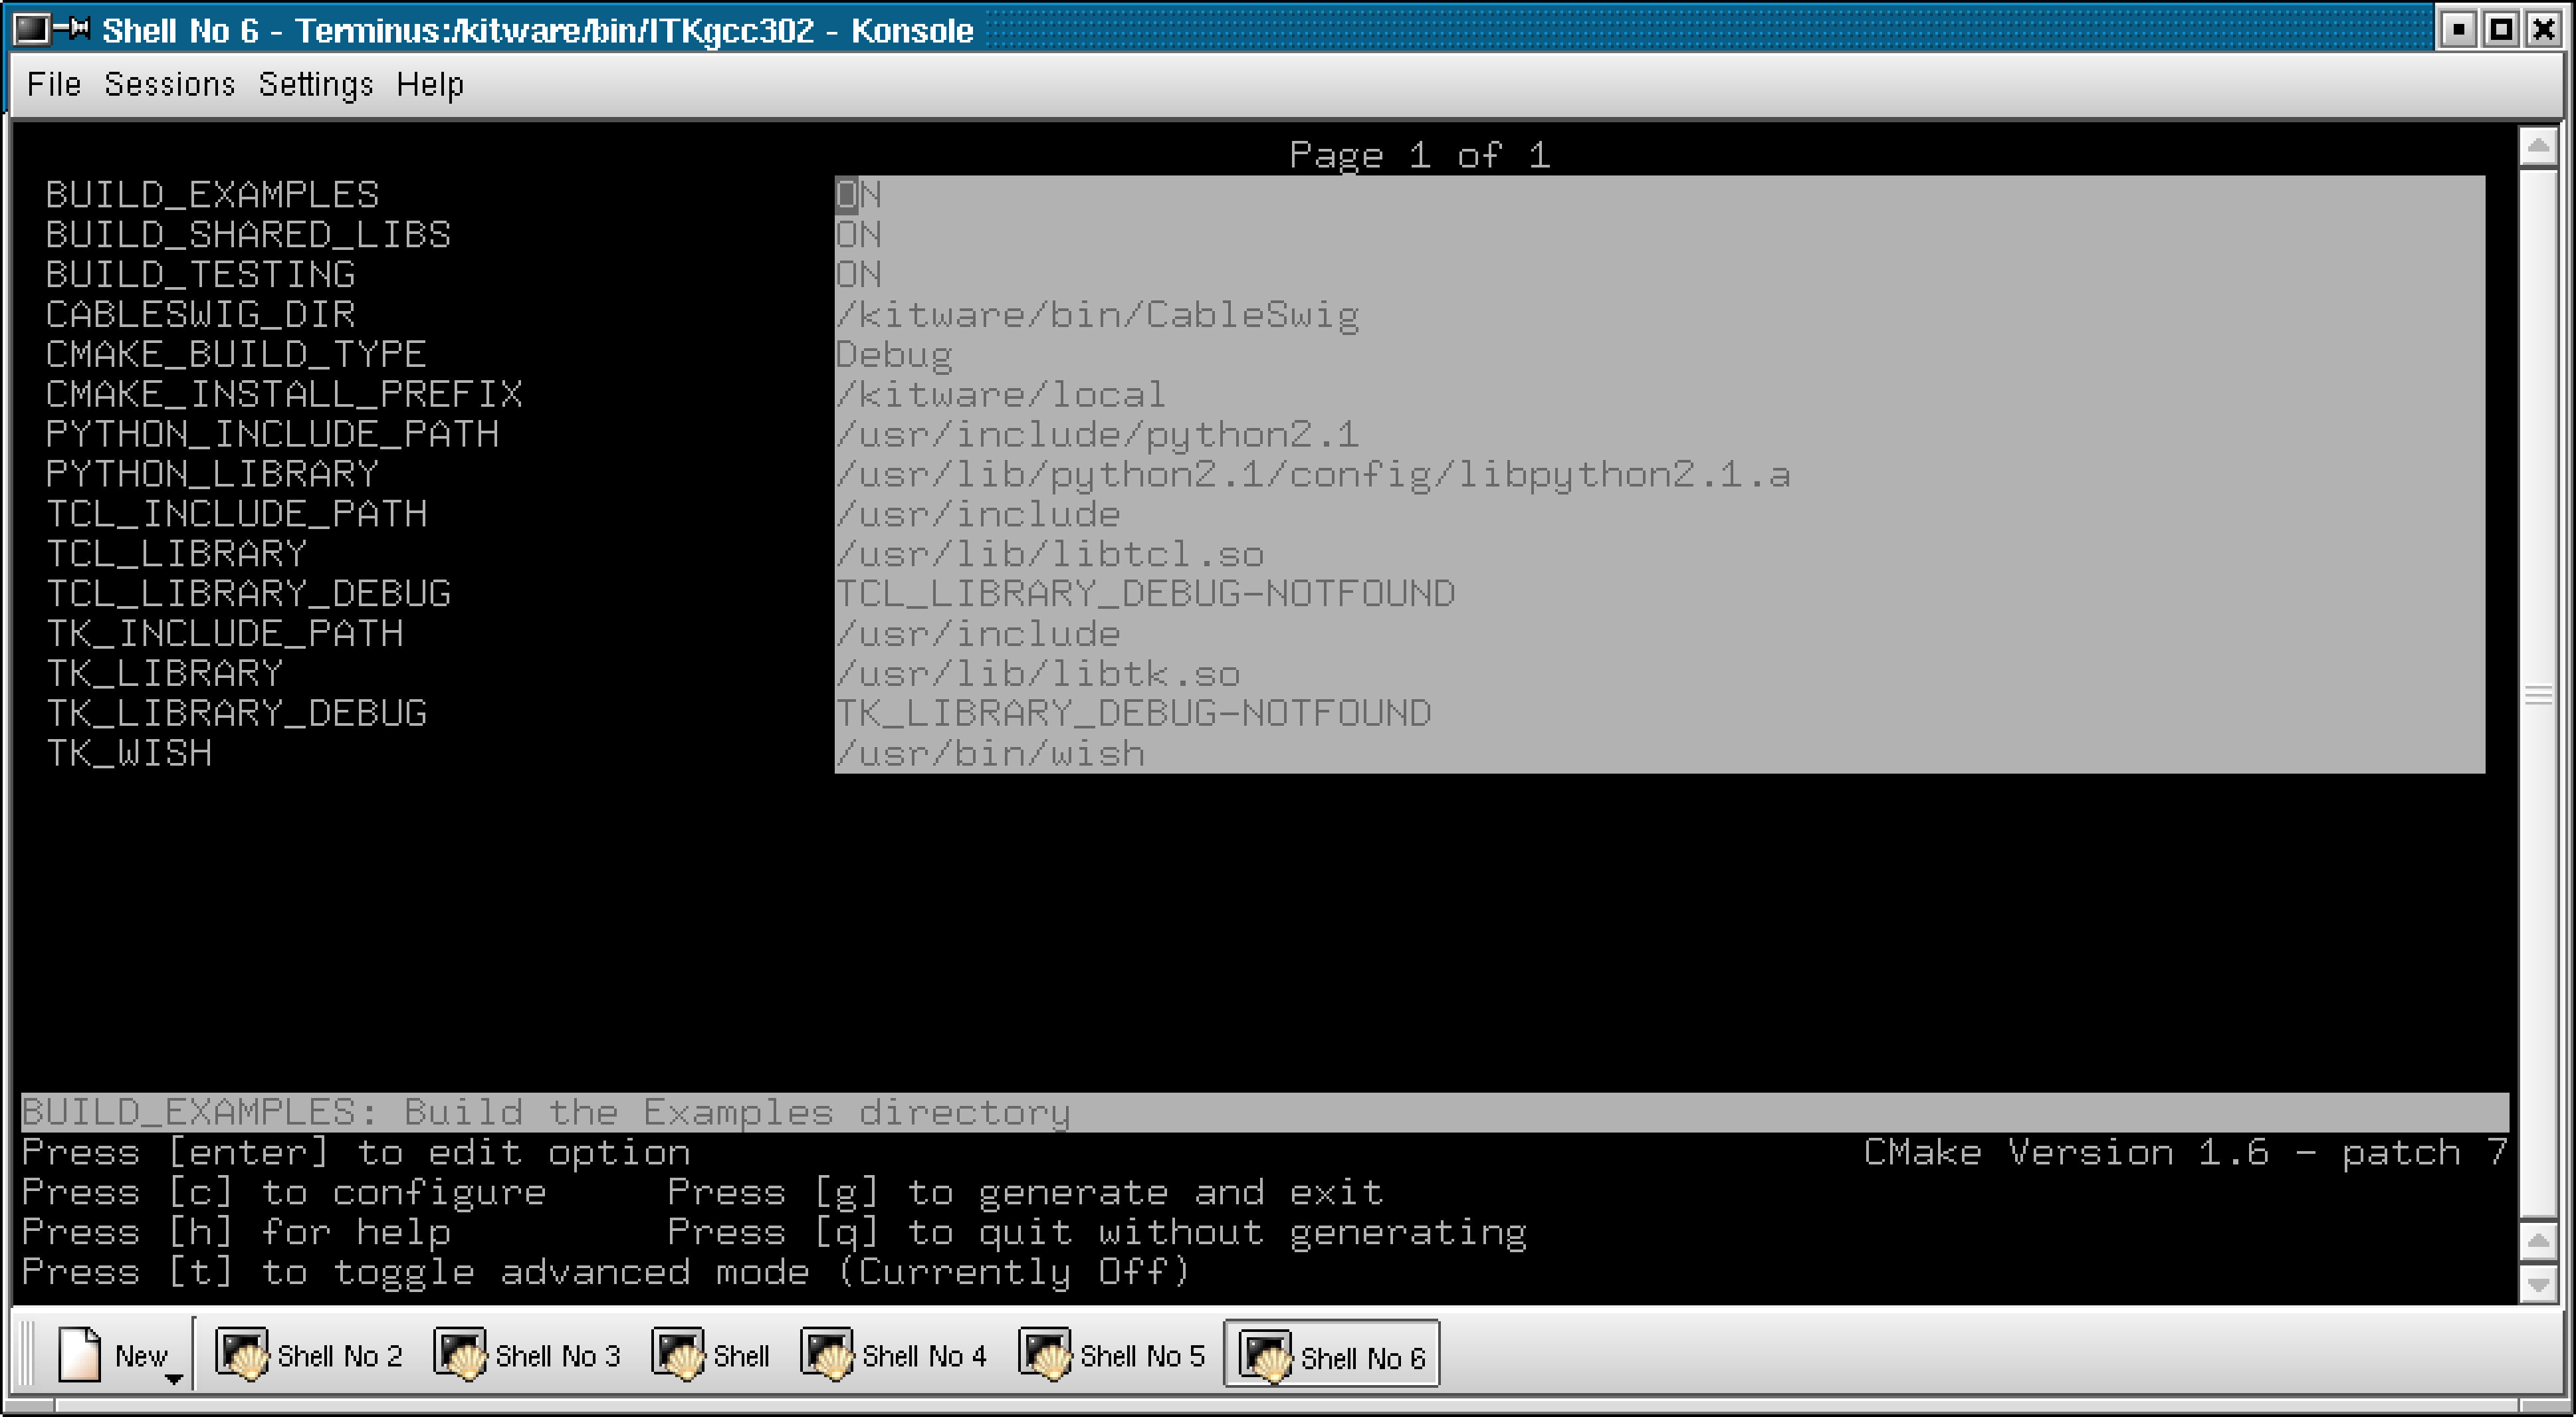
\includegraphics[height=0.45\textwidth]{ccmakeScreenShot.eps}
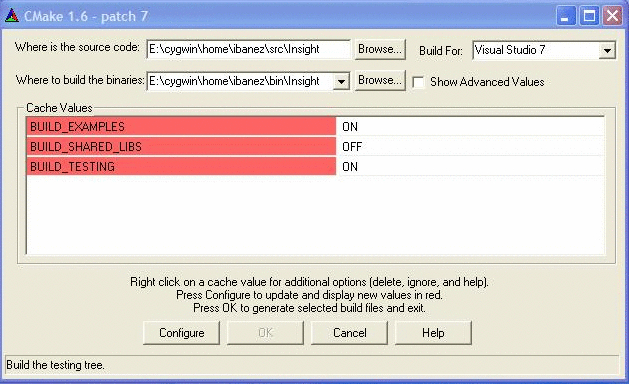
\includegraphics[height=0.45\textwidth]{CMakeSetupScreenShot.eps}
\caption{CMake interface. Left) \texttt{ccmake}, the UNIX version based on
\texttt{curses}. Right) \texttt{CMakeSetup}, the MS-Windows version based on MFC}
\label{fig:CMakeGUI}
\end{figure}

Figure \ref{fig:CMakeGUI} shows the CMake interface for UNIX and MS-Windows.
In order to speed up the build process you may want to disable the
compilation of the demo applications. This is done with the variable
\code{BUILD\_APPLICATIONS=OFF}. The demo applications  distributed with the
toolkit are a helpful resource for learning how to write problem-oriented
applications.  However, due to the large number of examples and the fact that
some of them rely on third party libraries that need to be installed and
configured, enabling this option will considerably complicate the initial
configuration of the toolkit.

Each time you change a set of variables in CMake, it is necessary to proceed
to another configuration step. In the Windows version this is done by
clicking on the ''Configure'' button. In the UNIX version this is done in a
\code{curses} interface where you can select to configure by hitting the
''c'' key.

When no new options appear in CMake, you can proceed to generate Makefiles or
Visual Studio projects. This is done in Windows by clicking on the ''Ok''
button.  In the UNIX version this is done by hitting the ''g'' key. After the
generation process is done CMake will quit silently. To initate the build
process, you can under UNIX simply type \code{make} while under Window you
will have to load the workspace named \code{ITK.dsw} from the directory that
you provide to CMake as Binary directory.

The build process will typically take from 30 minutes to one hour depending
on the performance of your system. As part of the normal built process, about
300 small test programs are compiled. This allows to verify that the basic
components of ITK have been correctly built on your system.

\section{Using ITK }
\label{sec:UsingITK}
 
The simplest way to get started with ITK is to create a new directory
somewhere in your disk and write two files on it. The first one is a
\code{CMakeList.txt} file which will be used by CMake to generate a Makefile
(if you are using UNIX) or a Visual Studio workspace (if you are using
MS-Windows).  The second file is an actual C++ file that will exercise some of
the multiple classes available in ITK.

Once both files are in your directory you can run CMake in order to configure
your project. Under UNIX, you can \code{cd} to your newly created directory
and type \code{"ccmake . "}. Note the "." in the command line for indicating
that the \code{CMakeList.txt} file is in the current directory. The
\code{curses} interface will require you to provide the directory where ITK
was built. This is the same path that you indicated for the
\code{ITK\_BINARY\_DIR} variable at the time of configuring ITK. Under
Windows you can run \code{CMakeSetup} and provide your newly created
directory as being both the source directory and the binary directory for
your new project. In CMake jargon this is called an
\emph{in-source} built. Then CMake will require you to provide the path to the
binary directory where ITK was built. The ITK binary directory should contain a
file named \code{UseITK.cmake} that was generated during the configuration
process at the time ITK was built.  From this file CMake will efficiently
recover all the information required to configure your new ITK project.  

\subsection{Hello World !}
\label{sec:HelloWorldITK}

\index{Hello World|textbf}

Here is the content of the two files to write in your new project. First, the
\code{CMakeList.txt} file.

\begin{verbatim}
PROJECT(HelloWorld)

INCLUDE (${CMAKE_ROOT}/Modules/FindITK.cmake)
IF (USE_ITK_FILE)
  INCLUDE(${USE_ITK_FILE})
ENDIF(USE_ITK_FILE)

ADD_EXECUTABLE(HelloWorld HelloWorld.cxx )

TARGET_LINK_LIBRARIES(HelloWorld ITKCommon)
\end{verbatim}

The first line will define the name of your project as it appears in Visual
Studio (it will have no effect under UNIX). The second line loads a CMake
file with a predefined strategy for finding ITK \footnote{Similar files are
provided in CMake for other commonly used libraries, all of them named
\code{Find*.cmake}}. If the strategy for finding ITK fails, CMake will prompt
you for the directory where ITK is installed in your system. In that case you
will write This information in the \code{ITK\_DIR} variable. The line \code{
INCLUDE(\${USE\_ITK\_FILE})} loads the UseITK.cmake file containing all the
configuration information from ITK. The \code{LINK\_LIBRARIES} line specify
which ITK libraries will be linked against this project. Finally the line
\code{ADD\_EXECUTABLE} defines as its first argument the name of the executable
that will be produced as result of this project. The following arguments in the
line are the names of the source files to be compiled and linked.

\input HelloWorld.tex

The Image class is explained in detail in section \ref{sec:ImageSection}.


